% The tools around a harness, and iChatBio beside it: what each piece is and
% which way text flows. Drawn for the tutorial in the book's figure style.
% ---------------------------------------------------------------------------
% style.tex --- shared preamble for every figure in book/figures/tikz/
%
% One style for all figures: Latin Modern, thin black lines, a light grey
% fill, and one accent colour used only to mark what is untrusted or wrong.
% Build with scripts/build_figures.sh; see book/figures/README.md.
% ---------------------------------------------------------------------------
\documentclass[tikz,border=6pt]{standalone}
\usepackage[T1]{fontenc}
\usepackage{lmodern}
\usetikzlibrary{arrows.meta,positioning,shapes.geometric,calc,fit,backgrounds}

\hyphenpenalty=10000   % short lines in boxes: ragged, never hyphenated

\definecolor{lightgrey}{gray}{0.92}
\definecolor{accent}{HTML}{9B2D20}

\tikzset{
  every picture/.style={
    line width=0.6pt,
    font=\small,
    >={Stealth[length=5pt,width=4pt]},
    node distance=14pt and 24pt,
  },
  % shapes
  box/.style={draw, rectangle, inner xsep=8pt, inner ysep=5pt,
              minimum height=22pt, align=center},
  grey/.style={box, fill=lightgrey},
  rounded/.style={box, rounded corners=9pt},
  decision/.style={draw, diamond, aspect=2.4, inner sep=1.5pt, align=center},
  group/.style={draw, dashed, rounded corners=5pt, inner sep=7pt},
  % text
  tag/.style={font=\footnotesize, align=center, inner sep=2pt},
  note/.style={font=\footnotesize\itshape, align=center, inner sep=2pt},
  code/.style={font=\small\ttfamily},
  codetag/.style={font=\footnotesize\ttfamily, align=center, inner sep=2pt},
  title/.style={font=\small\scshape, align=center, inner sep=2pt},
  % lines
  arrow/.style={->},
  back/.style={->, dashed},
  thin/.style={line width=0.4pt, gray},
  % the one accent, for what is untrusted, wrong or missing
  bad/.style={accent},
  badbox/.style={box, draw=accent, text=accent},
}

\begin{document}
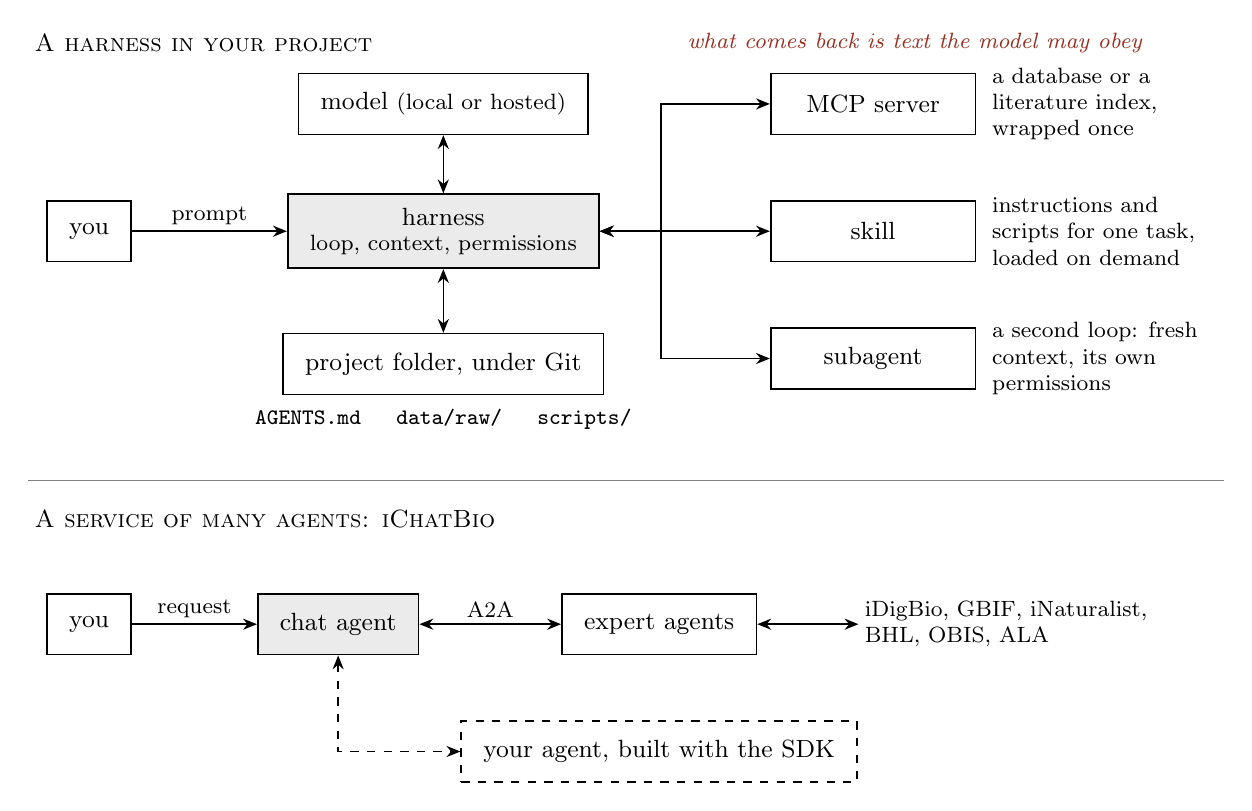
\begin{tikzpicture}
  % ---- Panel 1: a harness in your project ---------------------------------
  \node[title, anchor=west] at (0pt,172pt) {A harness in your project};
  \node[box] (you) at (22pt,104pt) {you};
  \node[grey, minimum width=112pt] (h) at (150pt,104pt)
    {harness\\[-2pt]{\footnotesize loop, context, permissions}};
  \node[box] (m) at (150pt,150pt) {model {\footnotesize (local or hosted)}};
  \node[box, minimum width=112pt] (git) at (150pt,56pt) {project folder, under Git};
  \node[codetag] at (150pt,36pt) {AGENTS.md \ \ data/raw/ \ \ scripts/};
  \draw[arrow] (you) -- node[tag, above] {prompt} (h);
  \draw[<->] (h) -- (m);
  \draw[<->] (h) -- (git);
  % the three things you can add
  \node[box, anchor=west, minimum width=74pt] (mcp) at (268pt,150pt) {MCP server};
  \node[box, anchor=west, minimum width=74pt] (sk)  at (268pt,104pt) {skill};
  \node[box, anchor=west, minimum width=74pt] (sub) at (268pt,58pt)  {subagent};
  \node[tag, anchor=west, align=left] at (346pt,150pt) {a database or a\\literature index,\\wrapped once};
  \node[tag, anchor=west, align=left] at (346pt,104pt) {instructions and\\scripts for one task,\\loaded on demand};
  \node[tag, anchor=west, align=left] at (346pt,58pt)  {a second loop: fresh\\context, its own\\permissions};
  \draw[<->] (h.east) -- ++(22pt,0) |- (mcp.west);
  \draw[<->] (h.east) -- (sk.west);
  \draw[<->] (h.east) -- ++(22pt,0) |- (sub.west);
  \node[note, bad, anchor=west] at (236pt,172pt) {what comes back is text the model may obey};
  % ---- Panel 2: iChatBio --------------------------------------------------
  \draw[thin] (0pt,14pt) -- (432pt,14pt);
  \node[title, anchor=west] at (0pt,0pt) {A service of many agents: iChatBio};
  \node[box] (you2) at (22pt,-38pt) {you};
  \node[grey] (chat) at (112pt,-38pt) {chat agent};
  \node[box] (exp) at (228pt,-38pt) {expert agents};
  \node[tag, anchor=west, align=left] (src) at (300pt,-38pt)
    {iDigBio, GBIF, iNaturalist,\\BHL, OBIS, ALA};
  \node[box, dashed] (yours) at (228pt,-84pt) {your agent, built with the SDK};
  \draw[arrow] (you2) -- node[tag, above] {request} (chat);
  \draw[<->] (chat) -- node[tag, above] {A2A} (exp);
  \draw[<->] (exp.east) -- (src.west);
  \draw[<->, dashed] (chat.south) |- (yours.west);
\end{tikzpicture}
\end{document}
